\documentclass[../thesis.tex]{subfiles}

\begin{document}
\chapter{Methods}
In this chapter, we will highlight the major methodological contributions that have been made in this thesis. The contributions fall into two major categories: how to infer label groups and how to train and make predictions from an HC. 

\section{Label Hierarchy Inference}
In our research when working with HCs, we have focused on the case where the label hierarchy is unknown potentially because there are too many labels for this partition to be created by hand or asking an expert for a label grouping would yield conflicting answers. Consequently, to employ an HC, the label grouping must be inferred from the data. The standard way to do this, as mentioned in Chapter 2, is to first trained a FC and then use spectral clustering on a validation matrix to infer the label groups. This approach has the advantage of tying the label hierarchy to classifier performance -- ultimately the most important metric -- however, this formulation requires that we first train a flat classifier, which somewhat defeats the point of pursuing this hierarchical approach and second to perform spectral clustering the user must provide the number of meta-classes a-priori. We address the first primary problem with spectral clustering with our two methods by employing k-means clustering and a mixed-integer programming formulation, and we tackle both of the problems when we propose a community detection based approach.

At the beginning of most of the label grouping methods we will discuss in this chapter, we will provide a diagram that visually depicts the underlying approach for this methodology. The purpose of these is to take what can be a quite abstract topic and make the methodology more understandable.

\subsection{K-Means Clustering}
Figure \ref{fig:ex-kmeans} depicts the overall process we will employ to utilize k-means clustering for providing label groupings: represent the labels as a single point and then perform k-means clustering on this representation of the data.

\begin{figure}
    \centering
    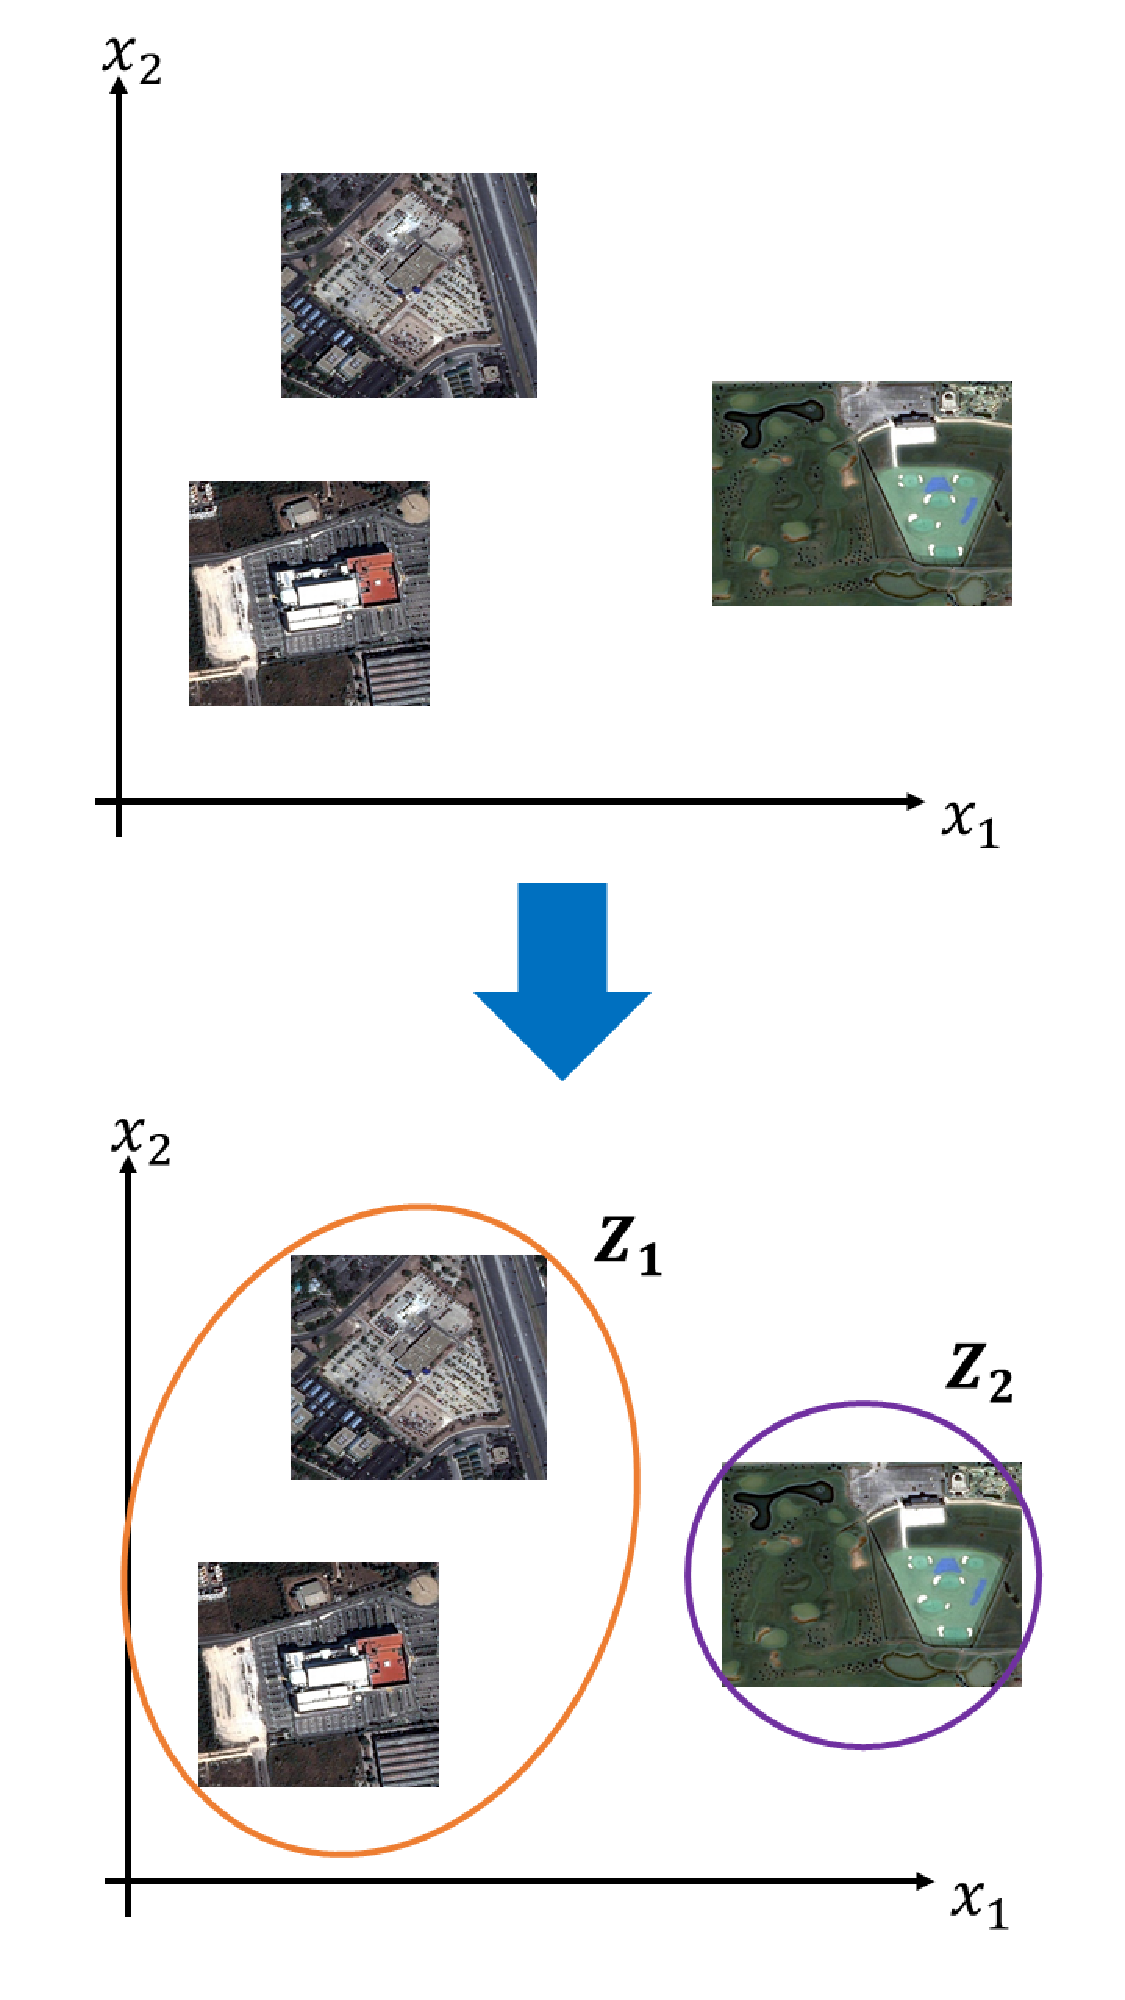
\includegraphics[width=.8\linewidth]{images/ex-kmeans.pdf}
    \caption[K-means Based Label Grouping]{This depicts an example of how the k-means algorithm is applied to group labels. In the first portion of the diagram, the three labels: shopping mall, car dealership, and golf course, are represented as a single point (in this case in two dimensions using principal component analysis for visualization purposes, but this is not necessary in general). Using the single points for the labels, the k-means clustering algorithm is then applied to generate the label groupings.}
    \label{fig:ex-kmeans}
\end{figure}

One of the major tasks of unsupervised machine learning is to find patterns in a data matrix, $\mathbf{X}$, by finding ``clusters'' or groups of similar data points. One of the most popular approaches to this task is an algorithm known as k-means clustering \cite{jain2010data}. This algorithm was first proposed in 1967 by James MacQueen in his paper, \textit{Some Methods for Classification and Analysis of Multivariate Observations} \cite{macqueen1967some}. Formulated as a mixed-integer program (MIP), k-means clustering attempts to solve
\begin{mini}
	{\textbf{z}, \boldsymbol{\mu}}{\sum_{i=1}^C \sum_{j=1}^L z_{ij} \lVert \mathbf{v}_i - \boldsymbol{\mu}_j \rVert_2^2}
	{\label{eq:minlp}}{}
	\addConstraint{\sum_j z_{ij}}{= 1}{\quad \quad \forall i}
	\addConstraint{\sum_i z_{ij}}{\geq 1}{\quad \quad \forall j}
	\addConstraint{z_{ij}}{\in \{0, 1\}}{\quad \quad \forall i,j}
\end{mini}
However, (\ref{eq:minlp}) is a integer, non-convex opptimization problem -- traditionally a very difficult class of problems to solve to provable optimiality \cite{burer2012non}. Instead of solving (\ref{eq:minlp}), the k-means clustering finds a locally optimal partition of the data points in $\mathbf{X}$. The standard algorithm was proposed by Stuart Lloyd in his paper, \textit{Least Squares Quantization in PCM}, where he proposes k-means clustering which has an ``assignment'' and ``update'' step \cite{lloyd1982least}. In the assignment step, the algorithm places data points in certain clusters by computing
\begin{equation}
    \label{eq:assign_step}
    S_i^t = \left \{ x_p : \lVert x_p - \mu_i^t \rVert_2^2 \leq \lVert x_p - \mu_j^t \rVert_2^2 \quad \forall j, 1 \leq j \leq k \right \}
\end{equation}
where $S_i^T$ and $\mu_i^t$ are the partition and centroid of the $i^{th}$ cluster at step $t$, respectively. In words what (\ref{eq:assign_step}) is saying is that we will move a data point, $x_p$ into the $i^{th}$ cluster if the distance from $x_p$ to $\mu_i^t$ is less than the distance of $x_p$ to the other cluster centroids. In the event where the distances between two centroids is the same, ties are broken arbitrarily. The second step of the k-means clustering algorithm is the update step where the centroids are given new values after various data points have been moved into different clusters. Mathematically this step corresponds to
\begin{equation}
    \label{eq:update_step}
    \mu_i^{t+1} = \frac{1}{|S_i^t|} \sum_{x_j \in S_j^t} x_j.
\end{equation}
In short, (\ref{eq:update_step}) is stating that the centroid of cluster $i$ is the average of the data points that have been moved into the partition during the assignment step. The algorithm has converged if no points have changed assignment; otherwise, the algorithm goes back to the assignment step. This algorithm does not guarantee a globally optimal solution because it solves the optimization problem proposed in (\ref{eq:minlp}) in a greedy fashion, but it is very popular in practice due to its speed and simplicity \cite{hartigan1979algorithm} \cite{jain2010data}.

Relating the k-means clustering algorithm to our problem, for our set-up we assume that we have both a data matrix, $\mathbf{X} \in \R^{n \times p}$ and labels $\mathbf{y} \in \{1, \ldots, C\}^n$; thus, this is by definition \textit{not} an unsupervised machine learning problem. However, the goal is to group similar labels with one another by using $\mathbf{X}$ and $\mathbf{y}$. Thus this can indeed be viewed as an unsupervised problem. 

Ultimately our goal is to infer some mapping matrix, $\mathbf{Z} \in \{0, 1\}^{C \times k}$ where $k$ is provided and which follows the constraints provided in (\ref{eq:minlp}). To this in a k-means clustering framework, we need to either have some way of back-tracking to the target from the clustering or we need to specifically encode a label as a single data point. 

A first cut at this problem would be to perform k-means clustering on the data matrix, $\mathbf{X}$, and then for each of the labels, determine the most common cluster assignment and map that label to the particular grouping. This approach is simple and easy to implement, but it does not guarantee that it will generate a feasible solution. For example, suppose that the number of labels, $C = 3$, and the number of meta-classes, $k=2$. \textbf{Insert diagram displaying extreme case of this approach. This could be the circles dictating the three labels and show how this can yield an infeasible solution.}

A better approach, and one that was first proposed by \cite{vural2004hierarchical}, is to represent each label using its mean sample -- like (\ref{eq:kmeans_mean}). Doing this for all labels, $j = 1, \ldots, C$, gives a matrix, $\mathbf{V} \in \R^{C \times p}$ where $\mathbf{v}_j$ represents the mean point for the $j^{th}$ label. Consequently performing k-means clustering on $\mathbf{V}$ will ensure that the resulting label map, $\mathbf{Z}$ is feasible. In this thesis we employ this k-means based approach as one of the techniques to infer a label hierarchy. This approach can summarized succinctly in two steps
\begin{enumerate}
    \item Build the $\mathbf{V}$ matrix by computing (\ref{eq:kmeans_mean}) for all labels, $j = 1, \ldots, C$
    \item Perform k-means clustering on $\mathbf{V}$.
\end{enumerate}

The benefits of this approach is that it is simple and allows us to generate a large number of candidate label hierarchies quickly. A simple question might be though: how is what we are doing any different than what was proposed by Vural and Dy in \cite{vural2004hierarchical}? The primary way we distinguish ourselves from \cite{vural2004hierarchical} is that we do not force force $k=2$; instead we treat the number of meta-classes as a hyper-parameter to be inferred using cross-validation. The reason that \cite{vural2004hierarchical} set $k=2$ and then recursively built the HC is that the authors were attempting to generate a new binary classifier which can compute test predictions more quickly. This is not our goal. Instead, we are interested in developing a HC which provides superior performance relative to a flat classifier and the standard spectral-clustering based approach to hierarchical classification. Second, if we were to force $k=2$, this requires us to make $\left \lceil \log_2(C) \right \rceil$ correct classifications to get the true label. The more correct classifications that have to be made, the higher the probability that an error will occur and thus propagate down the HC (this is also referred to as the ``routing problem'' and will be discussed later in this chapter). 

\subsection{Mixed-Integer Programming Formulation}
One of the biggest weak points of the k-means clustering algorithm is that it can stuck in bad local optima \cite{hartigan1979algorithm}. Common techniques to avoid this issue are to provide better starting centroids (most commonly done through the ``k-means++ algorithm'' \cite{arthur2007k}) and to perform a large number of random restarts \cite{dick2014many}. However, an area that has shown great research potential in recent years has been framing existing machine learning problems and formulating them as MIPs.  For example, this has been done with the best subset selection for a linear regression \cite{bertsimas2016best}, robust classification \cite{bertsimas2018robust}, and other common algorithms in ML. The initial research results from this effort has shown that by framing existing ML heuristics as MIPs, it possible to see significant out-of-sample improvements. Using this as a starting point, we proposed to frame the k-means clustering problem, as stated in (\ref{eq:minlp}) as a MIP to see if this could yield outcomes.

However, the objective function in (\ref{eq:minlp}) cannot be linearized since there is a quadratic term. Therefore instead of working with the $L_2$ norm, we proposed to solve
\begin{mini!}
	{\textbf{z}, \boldsymbol{\mu}}{\sum_{i=1}^C \sum_{j=1}^L z_{ij} \left(\sum_{k=1}^p |v_{ik} - \mu_{jk}|\right)}
	{\label{eq:milp1}}{}
	\addConstraint{\sum_j z_{ij}}{= 1}{\quad \quad \forall i}
	\addConstraint{\sum_i z_{ij}}{\geq 1}{\quad \quad \forall j}
	\addConstraint{z_{ij}}{\in \{0, 1\}}{\quad \quad \forall i,j}
\end{mini!}
By introducing an absolute value in the objective function of (\ref{eq:milp1}) it is now possible to linearize the formulation by converting the absolute value as well as the multiplication term in the objective.

To start since (\ref{eq:milp1}) is a minimization problem, the absolute value component of the MIP can be reformulated to form a linear decision variable. Specifically definite the auxiliary variable $\tau_{ijk} = |v_{ik} - \mu_{jk}$. By definition of an absolute value, the following conditions must hold
\begin{align}
    v_{ik} - \mu_{jk} &\leq \tau_{ijk} \quad \quad \forall i, j, k \label{eq:abs1} \\
    \mu_{jk} - v_{ik} &\leq \tau_{ijk} \quad \quad \forall i, j, k \label{eq:abs2}
\end{align}
Clearly the constraints (\ref{eq:abs1}) and (\ref{eq:abs2}) can be quite expensive given that we have three index sets to consider, but if the number of features $k$ is kept to small size, then the problem does not become unmanageable. Additionally, for notational simplicity, introduce the auxiliary variable $\gamma_{ij} = \sum_k \tau_{ijk}$. Combining these constraints and auxiliary variables we get the new formulation
\begin{mini!}
	{\textbf{z}, \boldsymbol{\mu}, \boldsymbol{\tau}, \boldsymbol{\gamma}}{\sum_{i, j} z_{ij} \gamma_{ij}}
	{\label{eq:milp2}}{}
	\addConstraint{\sum_j z_{ij}}{= 1}{\quad \quad \forall i}
	\addConstraint{\sum_i z_{ij}}{\geq 1}{\quad \quad \forall j}
	\addConstraint{v_{ik} - \mu_{jk}}{\leq \tau_{ijk}}{\quad \quad \forall i, j, k}
	\addConstraint{\mu_{jk} - v_{ik}}{\leq \tau_{ijk}}{\quad \quad \forall i, j, k}
	\addConstraint{\gamma_{ij}}{= \sum_k \tau_{ijk}}{\quad \quad \forall i, j}
	\addConstraint{z_{ij}}{\in \{0, 1\}}{\quad \quad \forall i,j}
\end{mini!}
However, (\ref{eq:milp2}) is still not a mixed-integer linear program (MILP) because there is a non-linearity in the objective function: $z_{ij} \gamma_{ij}$. This can be linearized by observing the following fact: by definition
\begin{equation*}
    \gamma_{ij} = \sum_k \tau_{ijk} = \left(\sum_k |v_{ik} - \mu_{jk}|\right) \geq 0.
\end{equation*}
This implies that $\gamma_{ij}$ is lower-bounded by zero and has an upper bound $M$ (we will discuss how we systematically go about finding this upper-bound later in this section). Consequently, we introduce the new constraints and auxiliary decision variables
\begin{align}
    \delta_{ij} &\leq Mz_{ij} \quad \quad \forall i, j \\
    \delta_{ij} &\leq \gamma_{ij} \quad \quad \forall i,j \\
    \delta_{ij} &\geq \gamma_{ij} - M(1-z_{ij}) \quad \quad \forall i, j \\
    \delta_{ij} &\geq 0 \quad \quad \forall i, j
\end{align}
Using these constraints we get the final, MILP formulation
\begin{mini!}
	{\textbf{z}, \boldsymbol{\mu}, \boldsymbol{\tau}, \boldsymbol{\gamma}, \boldsymbol{\delta}}{\sum_{i, j} \delta_{ij}}
	{\label{eq:milp3}}{}
	\addConstraint{\sum_j z_{ij}}{= 1}{\quad \quad \forall i}
	\addConstraint{\sum_i z_{ij}}{\geq 1}{\quad \quad \forall j}
	\addConstraint{v_{ik} - \mu_{jk}}{\leq \tau_{ijk}}{\quad \quad \forall i, j, k}
	\addConstraint{\mu_{jk} - v_{ik}}{\leq \tau_{ijk}}{\quad \quad \forall i, j, k}
	\addConstraint{\gamma_{ij}}{= \sum_k \tau_{ijk}}{\quad \quad \forall i, j}
	\addConstraint{\delta_{ij}}{\leq M z_{ij} \label{eq:big_m1}}{\quad \quad \forall i, j}
	\addConstraint{\delta_{ij}}{\leq \gamma_{ij}}{\quad \quad \forall i, j}
	\addConstraint{\delta_{ij}}{\geq \gamma_{ij} - M(1-z_{ij}) \label{eq:big_m2}}{\quad \quad \forall i, j}
	\addConstraint{\delta_{ij}}{\geq 0}{\quad \quad \forall i, j}
	\addConstraint{z_{ij}}{\in \{0, 1\}}{\quad \quad \forall i,j}
\end{mini!}
The MILP formulated in (\ref{eq:milp3}) can be quite large, particularly because of the triple index constraint for $\tau_{ijk}$. However, given that $L \ll C$, as long as the dimensionality of the data does not grow too rapidly, (\ref{eq:milp3}) can be solved by employing a linear relaxation heuristic discussed later in this section. However, before introducing the solution heuristic we must first discuss how to systematically find values for the big-$M$. 

\subsubsection{Big $M$ Procedure}
We mentioned earlier that we can upper-bound the value for $\gamma_{ij}$ with some value $M$, and it is important from a computational perspective that we are able to find this value because we do not want to cut off solutions by having an $M$ that is too small, but we also do not want to expand the search space either. We will now discuss a procedure where we can systematically find a way to upper-bound the value of $\gamma_{ij}$ such that we know we are not eliminating any solutions while simultaneously having the tightest upper-bound possible.

By definition $M$ corresponds to
\begin{equation*}
    M = \max \ \gamma_{ij} = \max \ \sum_k \tau_{ijk} = \max \ \left(\sum_k |v_{ik} - \mu_{jk}|\right).
\end{equation*}
Formally, I claim:

\begin{theorem}
    It is sufficient to find the $\max \ \left(\sum_k |v_{ik} - \mu_{jk}|\right)$ when $j = 1$ because the value is the same for every $j \in \{1, \ldots, L\}$.
\end{theorem}

\begin{proof}
    Suppose we have some vector $\mathbf{v}_i = (v_{i1}, v_{i2}, \ldots, v_{ip})^T$ and let $L$ be the number of meta-classes. Let $M_{ij}$ be the solution to the constrained optimization problem
    \begin{maxi}
    	{\boldsymbol{\mu}}{\sum_k |v_{ik} - \mu_{jk}|}
    	{\label{eq:big_m}}{}
    	\addConstraint{\mu_{jk}}{\geq L_k}{\quad \quad \forall k}
    	\addConstraint{\mu_{jk}}{\leq U_k}{\quad \quad \forall k}
    \end{maxi}
    where $L_k$ and $U_k$ define the lower and upper bounds of the data which is inferred from $\mathbf{V}$. We know these constraints must exist because in the original problem of finding the centroids which \textit{minimize} the $L_1$ distance, clearly the algorithm would never select a point $\mu_{jk}$ which was greater than $U_k$ or smaller than $L_k$. This is true because the objective value of (\ref{eq:milp1}) could be reduced by simply moving $\mu_{jk} = L_k$ if it was beyond the lower bound or $\mu_{jk} = U_k$ if it was greater than the upper bound. 
    
    Using this fact, we see that the constraints in (\ref{eq:big_m}) hold regardless of the meta-class index. That is, for every $j \in \{1, \ldots, L\}$ $\boldsymbol{\mu}_j$ is subject to the same constraints. This implies that (\ref{eq:big_m}) is the same optimization problem regardless of the meta-class index which necessarily means that
    \begin{equation*}
        \boldsymbol{\mu}_1 = \boldsymbol{\mu}_2 = \cdots = \boldsymbol{\mu}_L.
    \end{equation*}
    Therefore since we defined $M_{ij}$ as the solution to (\ref{eq:big_m}) this means that
    \begin{equation*}
        M_{i1} = M_{i2} = \cdots = M_{iL}.
    \end{equation*}
    Thus we know that it is sufficient to solve the optimization problem for $j = 1$ because $M_{ij}$ is the same for all $j$.
\end{proof}

Now that we have proved that the bound $M_{ij}$ is only dependent upon the given label $i$ and not the meta-class, $j$, we need to propose a way to find $M_i$ for every $i \in \{1, \ldots, C\}$. To do this, we will show a simple two-dimensional and show how we can easily infer what $M_i$ must be for a given label.

Suppose we have a $\mathbf{V}$ matrix equal to
\begin{equation*}
    \mathbf{V} =
    \begin{bmatrix}
        2 & 3 \\
        2 & 2 \\
        3 & 2 \\
        5 & 1 \\
    \end{bmatrix}
\end{equation*}
and we are interested in finding $M_1$ -- the max possible value for $\left(|v_{11} - \mu_{j1}| + |v_{12} - \mu_{j2}|\right)$. Using these values, we get the plot shown in Figure \ref{fig:big-m-plot} where $L_k$ and $U_k$ define the lower and upper bound for the $k^{th}$ dimension.

\begin{figure}
    \centering
    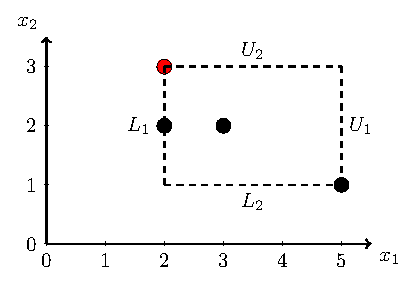
\includegraphics{images/big-m-plot.pdf}
    \caption[Big $M$ Inference Example]{This plot depicts a situation where there are four labels in two dimensions. Focusing specifically on the red label, the dashed lines depict the upper and lower bounds for the values of the data and the corresponding value for $M_1$ must exist on one of the four vertices of the rectangle as a consequence of minimizing an $L_1$ norm.}
    \label{fig:big-m-plot}
\end{figure}

In this instance, observe that $\mu_{j, 1} \in [2, 5]$ and $\mu_{j, 2} \in [1, 3]$. Since we are interested in maximizing the $L_1$ norm, it is sufficient to greedily find the maximum value for each dimension to determine $\mu_{jk}^*$ and then we can aggregate these value to compute $M_i$. Moreover, the maximum value for any given $\mu_{jk}^*$ must occur at the boundaries of the feasible set. This is true because one of the constraints in (\ref{eq:big_m}) must hold tightly at optimality because otherwise we could increase the objective function by making either the lower or upper bound constraint tight. Thus for the case of solving $M_1$, observe that $v_1 = (3, 2)$ and thus for $\mu_{j1}$ we can either select two or five and for $\mu_{j2}$ the options are one or three. Since we are interested in computing the upper bound for a given label we can greedily solve the optimization problems
\begin{equation*}
    m_{i1}^* = \underset{\{2, 5\}}{\text{max}} \ \left\{|2-2|, |2-5|\right\} = 3
\end{equation*}
and
\begin{equation*}
    m_{i2}^* = \underset{\{1, 3\}}{\text{max}} \ \left\{|3-1|, |3-3|\right\} = 2
\end{equation*}
where $m_{ik}^*$ is the maximal distance for the $k^{th}$ dimension for some point for the $i^{th}$ label. We then can get the final upper-bound $M_i$ by computing
\begin{equation}
    M_i = \sum_k m_{ik}^*.
\end{equation}

Ultimately the analysis we have conducted in this section allows us to write a very simple algorithm to compute the upper bound for each of the labels in the data set. 

\begin{algorithm}
    \caption{Upper-Bound Algorithm}
    \label{alg:upperbound}
    \begin{algorithmic}[1]
        \Procedure{find bounds}{$\mathbf{V}$}
            \For{$k \in \{1, \ldots, p$\}} \Comment{Get the upper and lower bounds for every $k$}
                \State $L_k \gets$ min $\left\{v_{1k}, \ldots, v_{Ck}\right\}$
                \State $U_k \gets$ max $\left\{v_{1k}, \ldots, v_{Ck}\right\}$
            \EndFor
            \For{$i \in \{1, \ldots, C\}$} \Comment{Compute $M_i$ for every $i$}
                \For{$k \in \{1, \ldots, p$\}}
                    \State $m_{ik}^* \gets$ max $\left\{|v_{ik} - L_k|, |v_{ik} - U_k|\right\}$
                \EndFor
                \State $M_i \gets \sum_k m_{ik}^*$
            \EndFor
            \State \textbf{return} $(M_1, \ldots, M_C)$
        \EndProcedure
    \end{algorithmic}
\end{algorithm}

Algorithm \ref{alg:upperbound} involves simply computing the upper and lower bounds for every dimension and then using those bounds to infer the largest possible value for a given label. We can therefore update the constraints (\ref{eq:big_m1}) and (\ref{eq:big_m2}) to be
\begin{align}
    \delta_{ij} &\leq M_i z_{ij} \quad \forall i, j \\
    \delta_{ij} &\geq \gamma_{ij} - M_i(1-z_{ij}) \quad \forall i, j
\end{align}
where instead of having a singular upper bound $M$ (which would be $M = \text{max} \left\{M_1, \ldots, M_C\right\}$), we instead can have a more refined bound for each class. As a consequence of employing this trick, we decrease the feasible region while maintaining the requirement that no feasible solutions be removed from the polyhedron.

\subsubsection{Linear Relaxation}
Even though we employed a number of linearization tricks to conver the MINLP, (\ref{eq:minlp}), into a MILP, oftentimes, (\ref{eq:milp3}), we still be quite difficult to solve, particularly because of the triple index auxiliary variable, $\tau_{ijk}$. This variable is dependent on both the number of classes and the desired number of label groupings as well as the dimensionality of the feature space which can be quite high. For example, the feature extract technique employed throughout the experiments yields a vector which has $4000+$ features. Therefore to be able to solve (\ref{eq:milp3}) in an appropriate amount of time, we employ a linear relaxation trick to convert the problem from a MILP to a standard linear program. 

The only integer variables in the formulation are the values $z_{ij}$ which denote whether the label $i$ has been placed in meta-class $j$. This is a binary variable and thus can be relaxed to a new variable, $z_{ij}^\prime \in [0, 1]$. However, since we are solving a LP approximation of the original MILP, we are not guaranteed to generate feasible solutions to the original problem and thus it is necessary to employ a conversion technique which will transform the LP solution into a feasible solution for the MILP in the event that the resulting partition matrix, $\mathbf{Z}$ does not yield all integer values. To develop such a conversion, let us briefly return to the original, non-linear formulation before we employed a number of linearization techniques. In (\ref{eq:minlp}) we have two primary variables of interest: the meta-class matrix, $\mathbf{Z}$, and the centroids of the label groupings: $\boldsymbol{\mu}$. Moreover, there are only two relevant constraints; in words these are:
\begin{enumerate}
    \item Every label must be assigned to a meta-class
    \item Every meta-class must contain at least one label
\end{enumerate}
For the feasible solution technique we will introduce, only the first constraint is necessary. Viewed differently, the constraints that $z_{ij} \in [0, 1]$ and $\sum_j z_{ij} = 1$ define a discrete probability distribution. Recall that a valid probability mass function for some random variable, $X$, has the following properties \cite{blitzstein2014introduction}:
\begin{enumerate}
    \item $\mathbf{P}(X = x) \geq 0$ for all $x \in X$
    \item $\sum_{x \in X} p_X(x) = 1$.
\end{enumerate}
For the linear relaxation of the (\ref{eq:milp3}), a row of the label grouping matrix, $\mathbf{z}_j$, can have non-negative mass for $L$ values of the vector, of which no value can be greater than one and the sum of the $L$ items must equal one. Thus, by definition a row of the partition matrix can be viewed as a probability distribution. Consequently this suggests that we can employ a sampling technique to generate feasible integer solutions. To make this concrete, we will start with a small example and then provide the overall algorithm.

Suppose that the linear relaxation for (\ref{eq:milp3}) for a problem with $C=3$ labels and $L=2$ meta-classes yielded the solution:
\begin{equation*}
    \mathbf{Z}^\prime = 
    \begin{bmatrix}
        0.67 & 0.33 \\
        1 & 0 \\
        0.5 & 0.5
    \end{bmatrix}
\end{equation*}
To generate integer feasible solutions from $\mathbf{Z}^\prime$, from the first row for instance, we could sample proportional to the ``distribution.'' Specifically, with probability $0.67$ we will place a one in the first column and with probability $0.33$ a one is placed in the second column. This same technique can be repeated for all of the other rows in $\mathbf{Z}^\prime$. Consequently this will generate a feasible integer solution (assuming that all of the columns have at least one entry in them). Moreover, this procedure can be done many times generating hundreds of unique, feasible integer solutions. The objective value of these solutions can then be computed and the one with the lowest error value can be treated as the final solution to the problem. There are further improvements that can be taken with this procedure (i.e., employing a local search to further refine the partition matrix), but this is discussed more in Chapter 6. 

The algorithm detailing this sampling procedure is shown in Algorithm \ref{alg:sampling-procedure}.

\begin{algorithm}
    \caption{Feasible Solution Generation}
    \label{alg:sampling-procedure}
    \begin{algorithmic}[1]
        \Procedure{Generate Solution}{$\mathbf{V}$, $n$}
            \State $\mathbf{Z}^\prime \gets$ Solution to linear relaxation of (\ref{eq:milp3})
            \State Define placeholder matrices $\{\mathbf{Z}^1, \ldots, \mathbf{Z}^n\}$ and placeholder objective values $\mathbf{s} = (\infty, \ldots, \infty)$
            \For{$i \in \{1, \ldots, n\}$}
                \For{$j \in \{1, \ldots, C\}$}
                    \State $l \gets $ Sample proportionally to $\mathbf{z}_j^\prime$
                    \State $Z^i_{jl} = 1$
                \EndFor
                \If{$\mathbf{Z}^i$ is not feasible} \Comment{Checking constraints in (\ref{eq:milp1})}
                    \State Discard $\mathbf{Z}^i$
                \Else{}
                    \State $\boldsymbol{\mu}^i \gets$ Infer from $\mathbf{V}$ and $\mathbf{Z}^i$
                    \State $\mathbf{s}_i \gets$ Compute objective using $\mathbf{Z}^i$ and $\boldsymbol{\mu}^i$
                \EndIf
            \EndFor
            \State $m^* \gets \argmin \{s_1, \ldots, s_n \}$
            \State \textbf{return} $\mathbf{Z}^{m^*}$
        \EndProcedure
    \end{algorithmic}
\end{algorithm}

Using Algorithm \ref{alg:sampling-procedure}, we can generate feasible label groupings in a computationally tractable manner.

\subsection{Community Detection}
Figure \ref{fig:ex-community-detection} depicts the process employed utilize community detection algorithms to infer label partitions: represent the labels as a graph using some similarity metric, and then use a community detection algorithm.

\begin{figure}
    \centering
    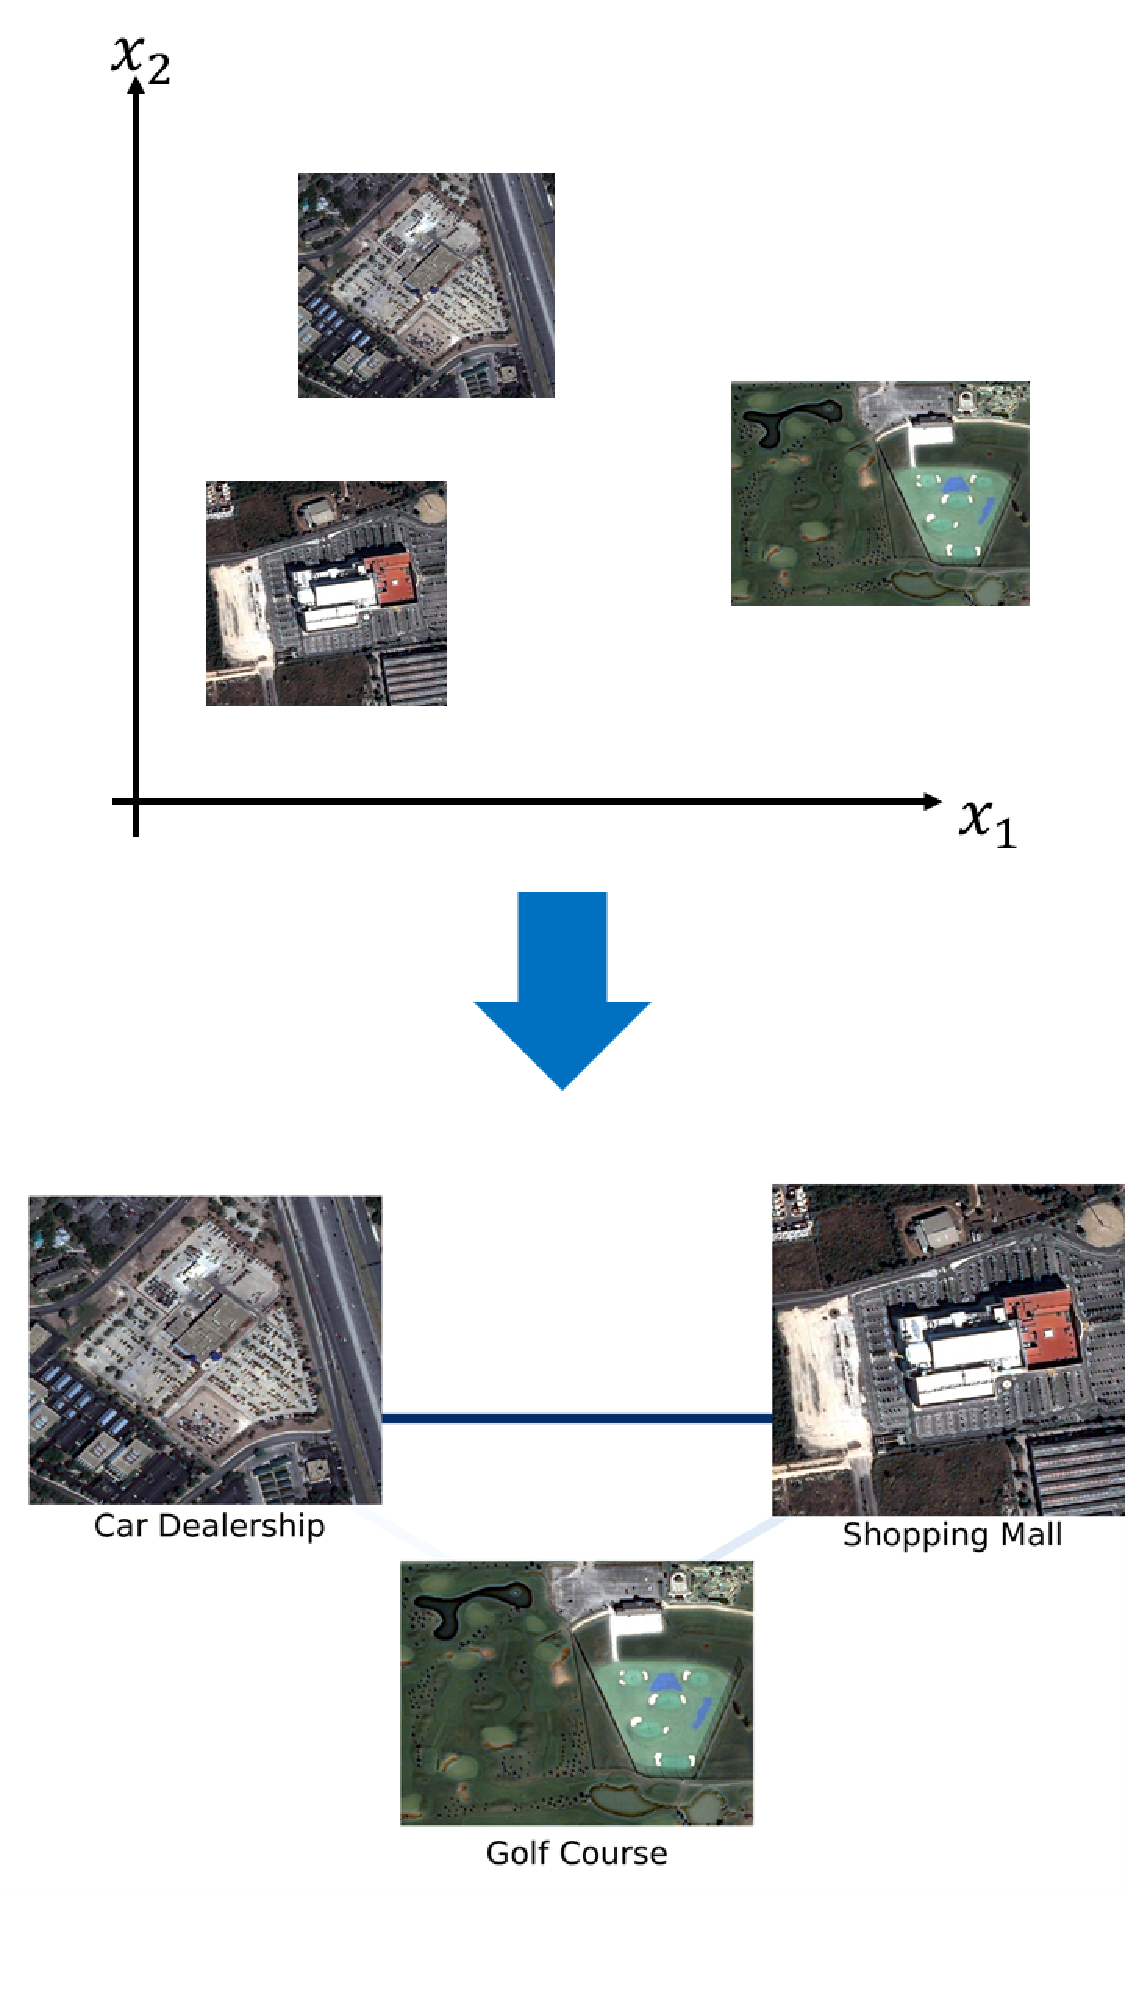
\includegraphics[width=.8\linewidth]{images/ex-community-detection.pdf}
    \caption[Community Detection Based Label Grouping]{This diagram the approach that we take to solve the label grouping problem using community detection. Like the k-means approach, we again represent the labels as single points. However, to employ a community detection algorithm we have to represent the labels as a graph. This is done by computing some similarity metric. The strength of the connection is denoted by the darkness of the edge in the figure}
    \label{fig:ex-community-detection}
\end{figure}

One of the major drawbacks of the employing either the k-means based approach or the MILP is that the user must specify the number of meta-classes in the data before using the algorithm. Consequently this requires the analyst to either know approximately how many groups are contained in the data beforehand or to treat this value as a hyper-parameter which inferred via cross-validation. The second case is the more typical approach because oftentimes one might know a reasonable range of values, but not the optimal number of label groupings. However, what if we did not have to specify the number of meta-classes? What if we had an algorithm that could infer this parameter automatically? This question motivates our third approach to the label grouping problem.

As we mentioned in Chapter \ref{modularity-max}, the objective of modularity-based community detection algorithms is to find locally optimal partition of nodes in a graph. The advantage of this approach is that we do not have to specify the number of communities in the graph. The algorithm, for this research the Louvain method, automatically infers this parameter. Thus for our problem of inferring the label hierarchy, to utilize these algorithms we must convert the data $\mathcal{D} = (\mathbf{X}, \mathbf{y})$ into a graph, represented by the affinity matrix, $\mathbf{A}$. Specifically, for the Louvain method to work, the values in the matrix must correspond to the degree of similarity between the labels. Since the algorithm is \textit{maximizing} modularity, a large value in the affinity matrix must correspond to a higher degree of similarity between those nodes. Thus to convert our data into the expected format we must define a similarity metric which meets these conditions and can be tractably computed. For this algorithm, we proposed four similarity metrics which one could use: the RBF kernel similarity, $L_2$ distance, $L_\infty$ distance, and the Wasserstein distance. We will go through each of these values, provide a justification for selecting them as a similarity metric, and then demonstrate how any of them can be used to accomplish the goal of representing the data as an affinity matrix.

\subsubsection{RBF Kernel Similarity}
As we introduced in (\ref{eq:rbf-kernel}), the RBF kernel is a metric which is used in a variety of settings. One of the most common applications for RBF kernels is using them for the ``kernel trick'' with support vector machines \cite{rahimi2008random}. However, and more relevant for our problem space, the value for the RBF kernel is defined between zero and one. The RBF kernel, $K(\mathbf{x}_i, \mathbf{x}_j) = 1$ when $\mathbf{x}_i = \mathbf{x}_j$, and it approaches zero asymptotically when the distance between the vectors increases. Thus the RBF kernel can be viewed as a similarity metric \cite{vert2004primer}.

The true way to compute the similarity between two class $i$ and $j$ would be to get all of the sample combinations in the set $\mathcal{M} = \{(i, j): i \in \mathbf{Y}_i, j \in \mathbf{Y}_j\}$ where $\mathbf{Y}_i$ and $\mathbf{Y}_j$ defines all of the samples for classes $i$ and $j$, respectively, and compute
\begin{equation}
    \label{eq:one-sim}
    s_{ij} = \frac{1}{|\mathcal{M}|} \sum_{(i, j) \in \mathcal{M}} K(\mathbf{x}_i, \mathbf{x}_j).
\end{equation}
Then to calculate the $s_{ij}$ values for every $(i, j)$ combination, there would have to be $\binom{C}{2}$ $s_{ij}$ computations.

To put this into context, one of the data sets which we utilized for experiments has $1013$ labels each of which has approximately $1000$ samples. Thus for a single $s_{ij}$ there would have to be $1000 \times 1000 = 1,000,000$ values that would have to be computed. Moreover, to repeat this procedure for all $1013$ labels, that would be $\binom{1013}{2} = 512,578$ pairs. Therefore a total of $512,578 \times 1,000,000 \approx 5 \times 10^{11}$ values which would need to be calculated. Since each sample in the data has $300$ features and the computations are assumed to be double precision, to calculate a single $s_{ij}$ value corresponds to approximately $2000$ floating point operations. Therefore in total compute the mean similarity between all $s_{ij}$ pairs there is approximately $5 \times 10^{11} \times 2000 \approx 1 \times 10^{15}$ floating point operations that would need to be performed. Moreover, the MIT Engaging cluster limits users to a total of $112$ processing cores each of which has a clock rate of $2.6$ GHz and can perform $16$ instructions per cycle. Therefore, at the absolute maximum -- ignoring all parallel overheads of communicating and synchronizing results -- we can calculate $112 \times 2.6 \text{GHz} \times 16 \approx 4.7$ TFLOPS. Thus using this strategy of doing all pairwise calculations completely in parallel, at best it would take $\frac{1 \times 10^{15}}{4.7 \times 10^9} \approx 212,765$ sec $\approx 59$ hours. Given that to fit a model takes on the order of tens to hundreds of minutes, clearly this strategy is computationally tractable. 

An alternative approach to computing the pairwise similarity between all labels is once again employ the $\mathbf{V}$ matrix which defines the mean point for each class. While there is still the price to pay calculating the $s_{ij}$ values for all $\binom{C}{2}$ target combinations, there is no longer the penalty of also calculating (\ref{eq:one-sim}). Using the previous example employing this strategy yields $\binom{1013}{2} \times 2000 \approx 1 \times 10^9$ floating point operations, which if we used the set-up all of the full CPU limit could be computed in approximately $0.2$ seconds. Thus, while we are sacrificing some accuracy of the similarity value between the labels, the difference in computational tractability clearly outweighs the cost.

Therefore, to employ the RBF kernel as the mechanism for representing the labels as an affinity matrix, $\mathbf{A}$, we simply first represent each target using the $\mathbf{V}$ matrix and then calculate the pairwise kernel for all $\binom{C}{2}$ targets. Because the value for the RBF kernel is defined between zero and one, this necessarily defines a similarity metric which can then be used by the Louvain method.

\subsection{Spectral Clustering Generalization}
In this final portion of the hierarchy inference, I will show how we can generalize the spectral clustering framework proposed by Bengio in \cite{bengio2010label} by using a HC as the warm-start.

\section{HC Training}
In this component of the methods section, I will describe the techniques we use to train a HC, assuming that the label hierarchy has already been inferred.

\subsection{Node-Level Features}
In this subsection, I will describe how we provide relevant features for each node in the HC. In particular we will describe how we used linear discriminant analysis (LDA) to provide relevant, supervised features to the node.

\subsection{Routing Problem}
Finally, I will describe how we compute posterior probabilities in a more robust way to avoid the ``routing problem'' that is traditionally seen with HCs. In particular, I will describe how using the LOTP allows us to compute better posterior probabilities versus simply using the arg-max prediction at a particular level. 

\section{Node Level Metrics}
For this section, I will introduce the metrics that we employ throughout our experiments to evaluate the performance of our classifiers. In particular I will first introduce the leaf-level metrics because they are easiest to understand. Afterwards, I will highlight how we developed the node-level metrics.

\subsection{Leaf-Level Metrics}
In this section, I will briefly introduce ``Leaf Top 1'' and ``Leaf Top 3.'' These are simple metrics which are commonly employed with other classifiers, so I don't expect that this will be a long discussion.

\subsection{Node-Level Metrics}
In this part of the methods section, I will introduce the node-level metrics that we created to help us compare HCs. In particular, I will discuss some of the challenges of comparing HCs and how we used the Monte Carlo based technique to attempt to skirt this issue. 

\end{document}